\section{HUMAN GESTURE}
\label{sec:gesture}

In this section, we propose a human gesture recognition system for the interaction system.
To achieve anytime{\-}anywhere startup of the palm landing motion, we need to consider a simple and intuitive gesture that can be easily recognized.
Looking back on falconry, falconers stretch their arm horizontally to use it as a landing port for the bird and bends the arm to stop the drone .
In other words, they switch the state of the bird from flying to landing by changing the relative position of the arm to the chest.
Inspired by this, we divide the drone states in midair into two: STAY and APPROACH,
and trigger the transition between them by the user's arm gesture.
The user bends the arm to stop the drone and stretches the arm to restart the drone as shown in Fig.~\ref{fig:flapper} and Fig.~\ref{fig:leg}.
To detect this gesture, we only need to measure the distance between the user's hand and chest $d$ and compare it with a threshold $d_{\text{th}}$.
The threshold $d_{\text{th}}$ can be interpreted as the minimum distance at which users can tolerate the drone's approach.
To determine the threshold, a previous study \cite{lieser2021evaluating-distances} can be referred to.
The study focuses on tactile drone interaction using a drone with a wheelbase of 0.92m, which is considered to be suitable for palm landing.
The study conducted an experiment in which participants were asked to stop the drone when they felt uncomfortable by using foot (non-contact) and hand (contact) methods.
It shows that even the minimum stop distance was above 0.30m, 
which means that the drone should not approach the user closer than this distance.
This indicates that physical contact should occur outside this range to guarantee physical and psychological safety.
Therefore, we set the threshold $d_{\text{th}}$ to 0.30m.

\begin{figure}
    \centering
    \begin{tabular}{cc}
        \begin{minipage}[t]{0.34 \columnwidth}
          \centering
          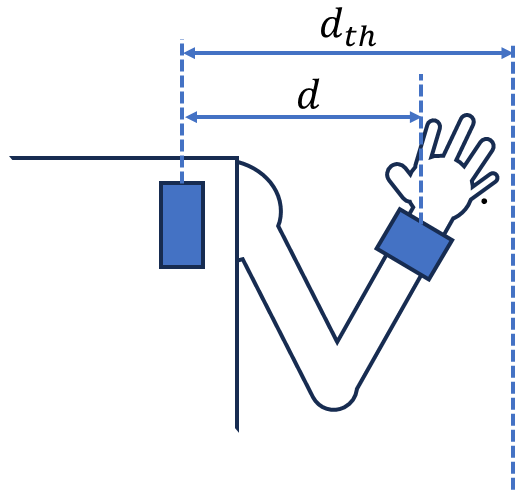
\includegraphics[keepaspectratio, scale=0.16]{bending.png}
          \subcaption{}
          \label{fig:flapper}
        \end{minipage} &
        \begin{minipage}[t]{0.48 \columnwidth}
          \centering
          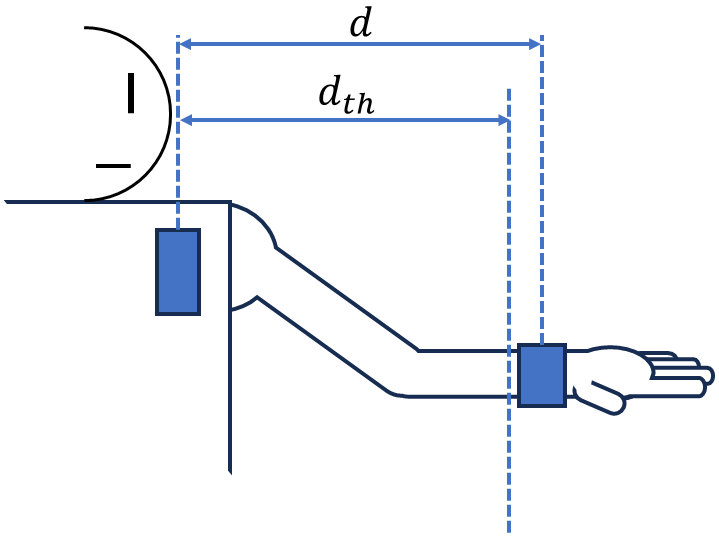
\includegraphics[keepaspectratio, scale=0.16]{stretching.png}
          \subcaption{}
          \label{fig:leg}
        \end{minipage}
      \end{tabular}
    \caption{Human gestures for the falconry-like interaction system. (a) Bending the arm to stop the drone. (b) Stretching the arm to start the approaching motion.}
    \label{fig:gesture}
  \end{figure}
